% !TEX TS-program = xelatex

\documentclass[13.5pt,aspectratio=169]{beamer}

\usepackage{polyglossia}
\setdefaultlanguage{spanish}

% Sets the background color to be light gray and the default text color to be heavy dark gray.
% Recommended for presenting with high quality projectors, since the high contrast of black-white is not advisable
\setbeamercolor{background canvas}{bg=colorlgray}
\setbeamercolor{normal text}{fg=colorhgray}


% personal data
\newcommand{\myTitle}{\color{colororange}\hugetext{AUTOENCODERS\\}{\notosansfont\largetext{teoría, herramientas y casos prácticos}}}
\newcommand{\myName}{\largetext{\color{colorblue}{David Charte}}\\\vspace{1em}%

\includegraphics[height=2em]{images/ugrhoriz.png}%
\hspace{1em}%

\includegraphics[height=2em]{images/sci2s.png}}
\newcommand{\myDetails}{\setnote{18 de diciembre de 2019}}

%sty file
\usepackage{config/presento}

% custom command and packages
% custom packages
\usepackage{textpos}
\setlength{\TPHorizModule}{1cm}
\setlength{\TPVertModule}{1cm}

\newcommand\crule[1][black]{\textcolor{#1}{\rule{2cm}{2cm}}}



\usetikzlibrary{shapes.misc, positioning, shapes.multipart, arrows.meta}
\tikzset{
    layer/.style={
        draw, 
        rectangle split,
        minimum width=2cm,
        rectangle split parts=3, 
        rectangle split part fill={black!10,white,black!10},
        rounded corners,
        inner sep=5pt,
    }
}

\hypersetup{
    colorlinks=false,% make the links colored
    linktoc=none% <- no links in ToC
}
\begin{document}
    \begin{frame}[plain]
  \vfill
    \myTitle
    \vfill
    \myName
    \vfill
    \myDetails
 \vfill
\end{frame}
    
    \begin{frame}{Índice}
      %{
         \tableofcontents
      %}
     \end{frame}
     
     \section{Fundamentos}
     \framecard[colororange]{{\color{white}\hugetext{FUNDAMENTOS}}}
     % 5 minutos
     \begin{frame}{Aprendizaje no supervisado}
      \begin{fullpageitemize}
        \item \textsc{\color{colorblue}definición}\\Búsqueda de patrones en datos sin etiquetar
        \item \textsc{\color{colorblue}motivación}\\Escasez de datos etiquetados,\\búsqueda de estructuras implícitas
        \item \textsc{\color{colorblue}métodos clásicos}\\K-medias (\textit{clustering}), LOF (anomalías)
   \end{fullpageitemize}
\end{frame}
     
     \begin{frame}{Aprendizaje de representaciones}
      \begin{fullpageitemize}
         % Demasiado texto
         % si no puedes recortar anade negrita
     %   \item {\montserratfont This is Montserrat}
     %   \item {\notosansfont This is Noto Sans}
     %   \item {\latolightfont This is Lato (light)}
     %   \item {\inconsolatafont This is inconsolata}
     %   \item \textsc{This is Alegreya Sans small caps}
     \item\textsc{\color{colorblue}motivación}\\Los modelos dependen de las variables\\Las representaciones mezclan factores que explican la variación
     \item\textsc{\color{colorblue}transformaciones clásicas}\\ Componentes principales, discriminantes lineales,\\escalado multidimensional, extracción de \textit{manifolds}
     \item\textsc{\color{colorblue}aplicaciones}\\Procesamiento de señales, reconocimiento de objetos, NLP, \textit{Transfer learning}
     \item\textsc{\color{colorblue}lectura recomendada}\\\textit{Representation Learning. A review and new perspectives} (Bengio {\scriptsize et al.})
   \end{fullpageitemize}
\end{frame}
     
     \begin{frame}{Redes neuronales}
      \begin{columns}
         \column{.5\linewidth}
         \begin{fullpageitemize}
            \item \begin{center}Capas de operaciones sencillas\end{center}
            \vspace{.2em}\item\begin{center}$+$\end{center}
            \vspace{.2em}\item \begin{center}Transformaciones no lineales\end{center}
            \vspace{.2em}\item\begin{center}$+$\end{center}%
            \vspace{.2em}\item \begin{center}Se propagan errores hacia atrás\end{center}
            \vspace{.2em}\item\begin{center}$+$\end{center}%
            \vspace{.2em}\item \begin{center}Se actualizan parámetros con SGD\end{center}%
      \end{fullpageitemize}
      \column{.5\linewidth}
      \textsc{\color{colorblue}claves}\\
      \begin{itemize}
         \item Cada capa extrae una representación\vspace{.5em}
         \item Una arquitectura es una familia paramétrica de funciones\vspace{.5em}
         \item El objetivo es diferenciable (c.p.d.)
      \end{itemize}

      \end{columns}
\end{frame}
     
     \begin{frame}{Autoencoders}
     
     \begin{columns}
      \begin{column}{.6\linewidth}
         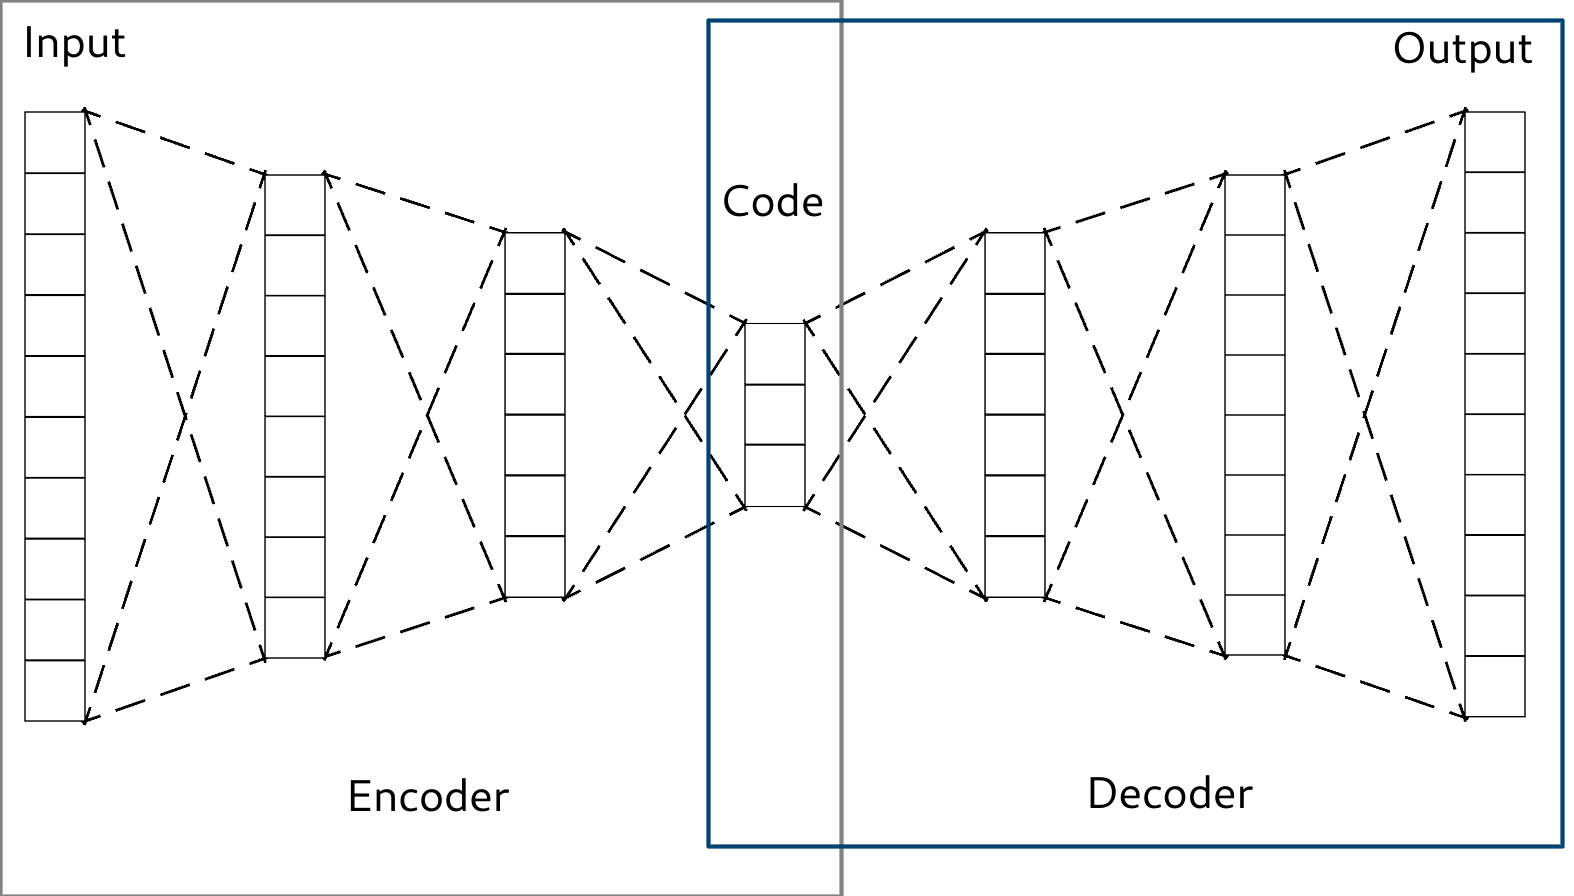
\includegraphics[width=\linewidth]{images/autoencoder.png}
      \end{column}%
      \begin{column}{.4\linewidth}
         Composición de un \textbf{\color{colorblue}codificador} y un \textbf{\color{colorblue}decodificador}.
         
         \vspace{1em}
         \textsc{\color{colorblue}objetivo}
         \[\min_{\theta}\sum_x d(c,g_{\theta}(f_{\theta}(x)))\]
      \end{column}
     \end{columns}
      \vfill
     \textsc{\color{colorblue}lectura recomendada}\\
     \textit{A practical tutorial on autoencoders for nonlinear feature fusion} (Charte {\scriptsize et al.})

     \end{frame}
     
     
     \section{Herramientas}
     \framecard[colororange]{{\color{white}\hugetext{HERRAMIENTAS}}}
     
     \begin{frame}[fragile]{Creación de un autoencoder}

      \textsc{\color{colorblue}tensorflow/keras}\\
      \begin{verbatim}
l_input     = Input(shape=(100,))
l_encoding  = Dense(10)(l_input)
l_code      = Input(shape=(10,))
l_decoding  = Dense(100)(l_code)
encoder     = Model(l_input, l_encoding)
decoder     = Model(l_code, l_decoding)
autoencoder = Model(l_input, decoder(l_encoding))
autoencoder.compile(optimizer="rmsprop", loss="mean_squared_error")\end{verbatim}

      \textsc{\color{colorblue}ruta} {\small(cran.r-project.org/package=ruta)}\\
      \begin{verbatim}
model = autoencoder(input() + dense(10) + output())
      \end{verbatim}
        % Demasiado texto
        % Estar'ia bien anadir negritas si no
     \end{frame}
     
     \begin{frame}{Implementaciones}
      \begin{fullpageitemize}
      \item\textsc{\color{colorblue}ruta} {\small\url{ruta.software}}\\
      Autoencoders denso, convolucional $+$\\\textit{sparse}, \textit{\textbf{\color{colorblue}contractive}},  \textit{denoising}, \textit{robust}, \textit{\textbf{\color{colorblue}variational}}
      

      \item\textsc{\color{colorblue}autoencoder} {\small\url{pypi.org/project/autoencoder/}}\\
      Autoencoder convolucional personalizable

      \item\textsc{\color{colorblue}keras} {\small\url{github.com/keras-team/keras/blob/master/examples/variational\_autoencoder\_deconv.py}}\\
      Autoencoder variacional convolucional (MNIST)

      \item\textsc{\color{colorblue}seq2seq} {\small\url{pypi.org/project/seq2seq}}\\
      Encoder-decoder para secuencias reales

      
        
      \end{fullpageitemize}
     \end{frame}
     \section{Casos prácticos}
        
     \framecard[colororange]{{\color{white}\hugetext{CASOS PRÁCTICOS}}}
     % Resumen del paper de neucom
     \begin{frame}{Embedding}
        \begin{figure}[ht]
           \centering\small
           \resizebox{\linewidth}{!}{
               \begin{tikzpicture}[node distance=0.5cm]
                   \node[layer] (x) {\textsc{input}
                   \nodepart{second} CPU Activity
                   \nodepart{third} 21};
                   \node[layer, right=of x] (h1) {\textsc{}
                   \nodepart{second} Dense
                   \nodepart{third} 6};
                   \node[layer, right=of h1] (h3) {\textsc{encoding}
                   \nodepart{second} Dense
                   \nodepart{third} 2};
                   \node[layer, right=of h3] (h4) {\textsc{}
                   \nodepart{second} Dense
                   \nodepart{third} 6};
                   \node[layer, right=of h4] (y) {\textsc{output}
                   \nodepart{second} Dense
                   \nodepart{third} 21};
                   \draw[-Latex] (x.east) to (h1.west);
                   \draw[-Latex] (h1.east) to (h3.west);
                   \draw[-Latex] (h3.east) to (h4.west);
                   \draw[-Latex] (h4.east) to (y.west);
                   \node[layer, right=of y] (xx) {\textsc{input}
                   \nodepart{second} Satellite
                   \nodepart{third} 36};
                   \node[layer, right=of xx] (z1) {\textsc{}
                   \nodepart{second} Dense
                   \nodepart{third} 8};
                   \node[layer, right=of z1] (z3) {\textsc{encoding}
                   \nodepart{second} Dense
                   \nodepart{third} 2};
                   \node[layer, right=of z3] (z4) {\textsc{}
                   \nodepart{second} Dense
                   \nodepart{third} 8};
                   \node[layer, right=of z4] (yy) {\textsc{output}
                   \nodepart{second} Dense
                   \nodepart{third} 36};
                   \draw[-Latex] (xx.east) to (z1.west);
                   \draw[-Latex] (z1.east) to (z3.west);
                   \draw[-Latex] (z3.east) to (z4.west);
                   \draw[-Latex] (z4.east) to (yy.west);
                   \end{tikzpicture}        
           }
           \label{fig:visualizer}
       \end{figure}
     \begin{figure}[ht!]
        \centering
     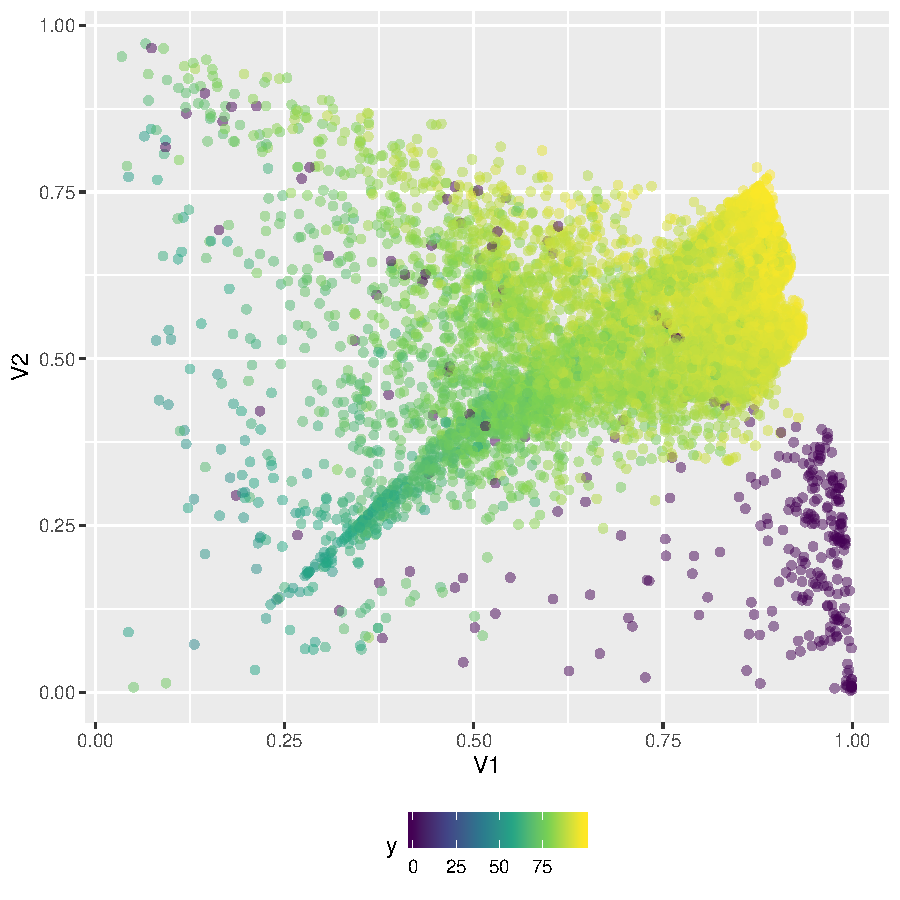
\includegraphics[width=.4\linewidth]{images/visualization_cpu}%
     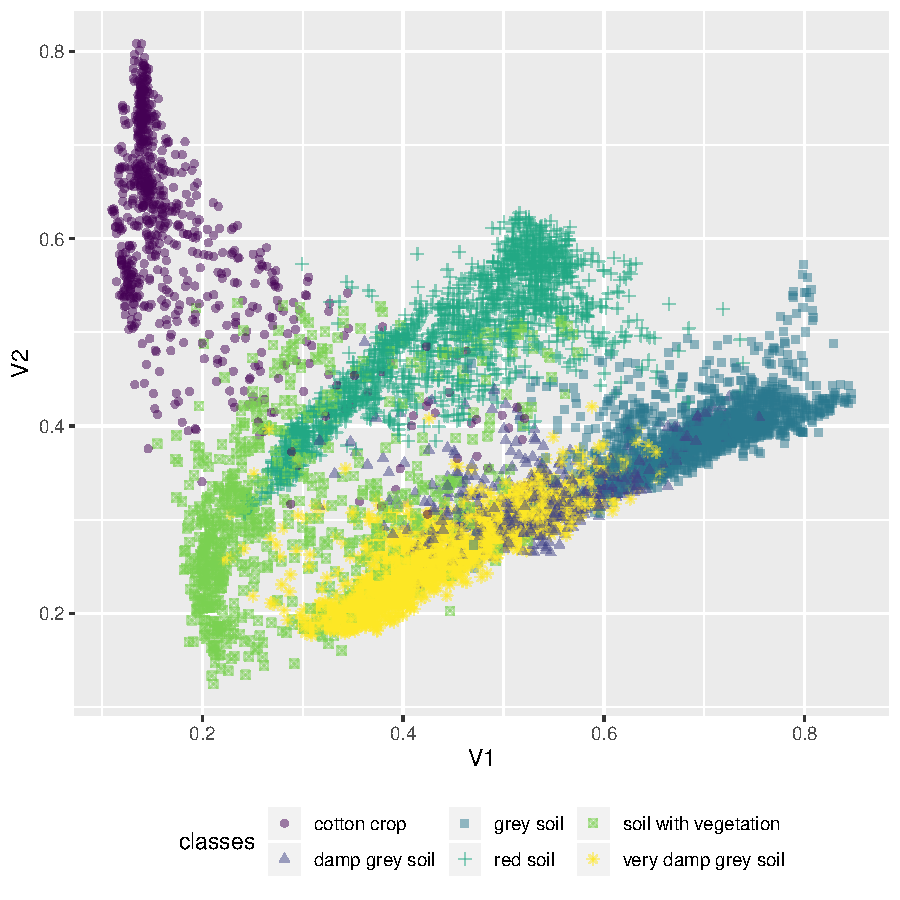
\includegraphics[width=.4\linewidth]{images/visualization_sat2}
        \label{fig:visualizations}
     \end{figure}
     \end{frame}
     \begin{frame}[fragile]{Ajuste de distribuciones (I): instance generation}
        
        \begin{columns}
           \begin{column}{.3\linewidth}\centering
            \textbf{\color{colorblue}Variational AE}: 
           \end{column}
           \begin{column}{.7\linewidth}
              
        \resizebox{\linewidth}{!}{%
        \begin{tikzpicture}[node distance=0.5cm]
        \node[layer] (x) {\textsc{input}
        \nodepart{second} AT\&T faces
        \nodepart{third} $ 64 \times 64\times 1 $};
        \node[layer, right=of x] (h1) {\textsc{}
        \nodepart{second} Conv ($3 \times 3$)
        \nodepart{third} $ 32 \times 32 \times 8 $};
        \node[layer, right=of h1] (h2) {\textsc{}
        \nodepart{second} Conv ($3 \times 3$)
        \nodepart{third} $ 16 \times 16 \times 16 $};
        \node[layer, right=of h2] (h3) {\textsc{}
        \nodepart{second} Conv ($3 \times 3$)
        \nodepart{third} $ 8 \times 8 \times 32 $};
        \node[layer, right=of h3] (h4) {\textsc{mean \& var}
        \nodepart{second} Dense
        \nodepart{third} $ 32 + 32 $};
        \node[layer, right=of h4] (h5) {\textsc{sampling}
        \nodepart{second} Custom
        \nodepart{third} $ 32 $};
        \node[layer, below=of h5] (h6) {\textsc{}
        \nodepart{second} Dense
        \nodepart{third} $ 8 \times 8 \times 8 $};
        \node[layer, left=of h6] (h7) {\textsc{}
        \nodepart{second} Deconv ($3 \times 3$)
        \nodepart{third} $ 16 \times 16 \times 32 $};
        \node[layer, left=of h7] (h8) {\textsc{}
        \nodepart{second} Deconv ($3 \times 3$)
        \nodepart{third} $ 32 \times 32 \times 16 $};
        \node[layer, left=of h8] (h9) {\textsc{}
        \nodepart{second} Deconv ($3 \times 3$)
        \nodepart{third} $ 64 \times 64 \times 8 $};
        \node[layer, left=of h9] (y) {\textsc{output}
        \nodepart{second} Deconv ($3 \times 3$)
        \nodepart{third} $ 64 \times 64 \times 1 $};
        \draw[-Latex] (x.east) to (h1.west);
        \draw[-Latex] (h1.east) to (h2.west);
        \draw[-Latex] (h2.east) to (h3.west);
        \draw[-Latex] (h3.east) to (h4.west);
        \draw[-Latex] (h4.east) to (h5.west);
        \draw[-Latex] (h5.south) to (h6.north);
        \draw[-Latex] (h6.west) to (h7.east);
        \draw[-Latex] (h7.west) to (h8.east);
        \draw[-Latex] (h8.west) to (h9.east);
        \draw[-Latex] (h9.west) to (y.east);
        \end{tikzpicture}
        }
           \end{column}
        \end{columns}
     
     \begin{columns}
        \begin{column}{.6\linewidth}
           
\scriptsize\begin{verbatim}
   cross_ent = tf.nn.sigmoid_cross_entropy_with_logits(
         logits=predictions, labels=inputs)
   logpx_z = -tf.reduce_sum(cross_ent, axis=[1, 2])
   logpz = log_normal_pdf(z, 0., 1.)
   logqz_x = log_normal_pdf(z, mean, logvar)
   variational_loss = -tf.reduce_mean(10*logpx_z + logpz - logqz_x)
   \end{verbatim}\normalsize
        \end{column}\hfill
        \begin{column}{.3\linewidth}

         \begin{figure}[ht!]
            \centering
            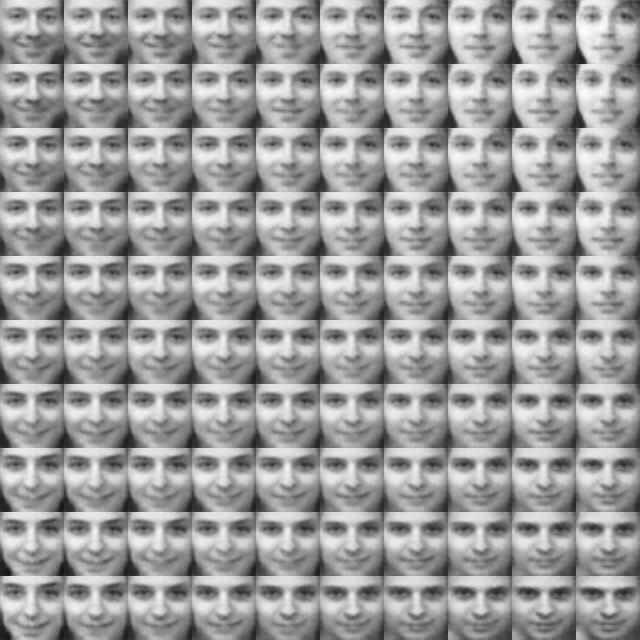
\includegraphics[width=\linewidth]{images/variational-matrix.png}
         \label{fig:sampledfaces}
         \end{figure}           
        \end{column}
     \end{columns}

     \end{frame}
     \begin{frame}{Ajuste de distribuciones (II): feature disentanglement}
      \centering
        \textbf{\color{colorblue}Adversarial AE} = AE + GAN
     
     \begin{figure}[ht!]
        \centering\hfill
        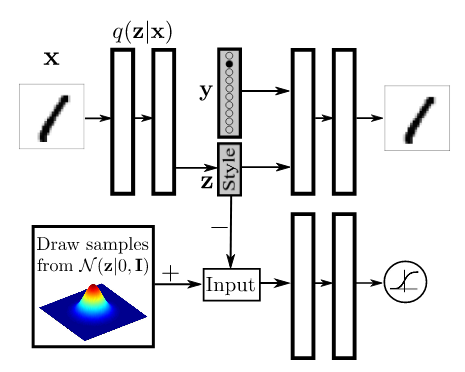
\includegraphics[height=.3\linewidth]{images/supaae.png}\hfill
        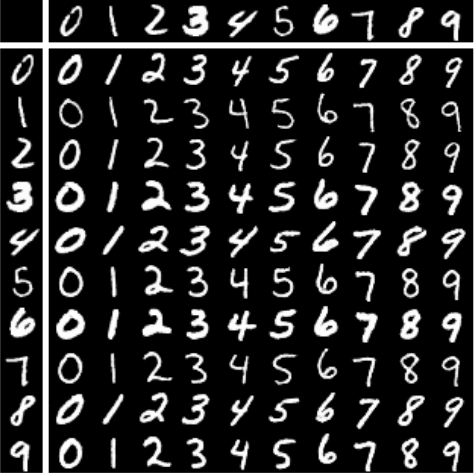
\includegraphics[height=.3\linewidth]{images/ae-disentange.png}\hfill
     \label{fig:sampledfaces}
     \end{figure}\flushleft
     \textsc{\color{colorblue}lectura recomendada}\\
     \textit{Adversarial Autoencoders} (Makhzani {\scriptsize et al.})
     \end{frame}
     \begin{frame}{Limpieza}
        
     \begin{figure}[ht]
      \centering\small
       \resizebox{\linewidth}{!}{
   \begin{tikzpicture}[node distance=0.5cm]
   \node[layer] (x) {\textsc{input}
   \nodepart{second} STL10 + noise
   \nodepart{third} $96\times 96\times 3$};
   \node[layer, right=of x] (h1) {\textsc{}
   \nodepart{second} Conv ($5\times 5$)
   \nodepart{third} $96\times 96\times 64$};
   \node[layer, right=of h1] (h2) {\textsc{}
   \nodepart{second} Conv ($1\times 1$)
   \nodepart{third} $96\times 96\times 128$};
   \node[layer, right=of h2] (h3) {\textsc{Encoding}
   \nodepart{second} Max pooling ($2\times 2$)
   \nodepart{third} $48\times 48\times 128$};
   \node[layer, right=of h3] (h5) {\textsc{}
   \nodepart{second} Deconv ($5\times 5$)
   \nodepart{third} $48\times 48\times 64$};
   \node[layer, right=of h5] (h6) {\textsc{}
   \nodepart{second} Upsampling ($2\times 2$)
   \nodepart{third} $96\times 96\times 64$};
   \node[layer, right=of h6] (y) {\textsc{output}
   \nodepart{second}  Deconv ($3\times 3$)
   \nodepart{third} $96\times 96\times 3$};
   \draw[-Latex] (x.east) to (h1.west);
   \draw[-Latex] (h1.east) to (h2.west);
   \draw[-Latex] (h2.east) to (h3.west);
   \draw[-Latex] (h3.east) to (h5.west);
   \draw[-Latex] (h5.east) to (h6.west);
   \draw[-Latex] (h6.east) to (y.west);
   \end{tikzpicture}
   }
      \label{fig:graph-denoising}
   \end{figure}
   
   \begin{figure}[ht]
      \centering
      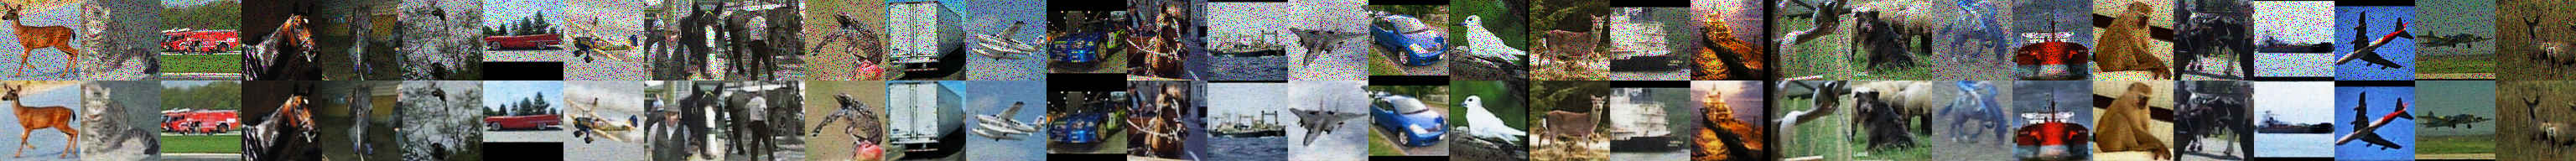
\includegraphics[width=\linewidth,trim={1445pt 0 780pt 0},clip]{images/denoising-predictions.png}
   \end{figure}
     \end{frame}
     \begin{frame}{Otras aplicaciones}
      \begin{fullpageitemize}
         \item \textbf{\color{colorblue}Superresolución} de imágenes
         \item \textbf{\color{colorblue}Compresión} de imágenes y señales
         \item \textbf{\color{colorblue}Hashing} semántico
         \item \textit{\textbf{\color{colorblue}Transfer} learning}
         \item Recuperación de \textbf{\color{colorblue}poses} humanas
         \item Aprendizaje de \textbf{\color{colorblue}formas 3D}
         \item Sistemas de \textbf{\color{colorblue}recomendación} y etiquetado
      \end{fullpageitemize}
        
     \end{frame}
     
     \section{Detección de anomalías}
     \framecard[colororange]{{\color{white}\hugetext{DETECCIÓN DE ANOMALÍAS}}}
     
     \begin{frame}{Estrategia}
      \begin{columns}
         \column{0.5\linewidth}
         \begin{fullpageitemize}
            \item \textsc{\color{colorblue}conjetura}\\Un autoencoder entrenado en datos normales no puede reconstruir datos anómalos\vspace{1em}
            \item \textsc{\color{colorblue}método}\\Score = error de reconstrucción\vspace{1em}
            \item \textsc{\color{colorblue}lectura recomendada}\\
            {\small\textit{Anomaly detection using autoencoders with nonlinear dimensionality reduction} (Sakurada {\scriptsize et al.})}
         \end{fullpageitemize}
         \column{0.5\linewidth}
         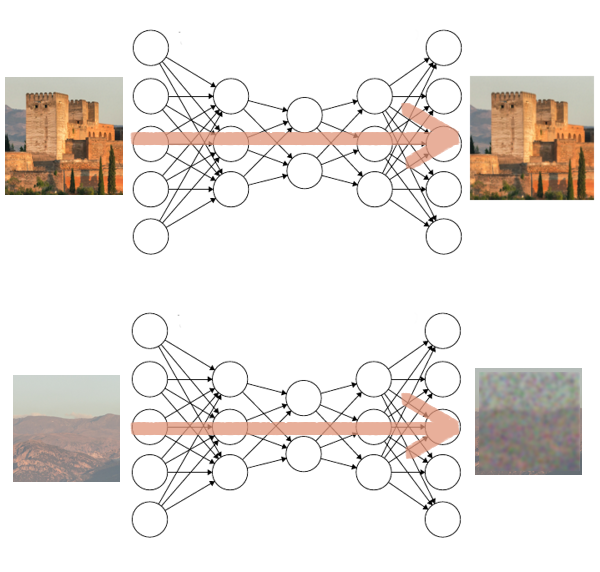
\includegraphics[width=\linewidth]{images/autoencoders-anom.png}
      \end{columns}
      

     \end{frame}
     
     \begin{frame}[fragile]{Implementación}

        Detección de ataques en redes: \textbf{\textcolor{colorblue}{UNSW-NB15}}

        \begin{verbatim}
autoencoder = Sequential([
  Dense(units=2, input_shape=187, activation="relu"),
  Dense(units=187)
])
autoencoder.compile(loss="mean_squared_error", optimizer="adam")
autoencoder.fit(train_x, train_x, epochs=5, batch_size=256)

rec = autoencoder.predict(test_x)
train_rec = autoencoder.predict(train_x)

# cálculo de errores...
        \end{verbatim}
        
         
     \end{frame}

     \begin{frame}{Resultados}
        
      \includegraphics[width=.5\linewidth]{images/anomaly_column.eps}%
      \includegraphics[width=.5\linewidth]{images/anomaly_histogram.eps}
     \end{frame}

     \begin{frame}{Extensiones}
      \begin{columns}
         \begin{column}{.3\linewidth}
            \begin{itemize}
               \item[1.] Variacional\vspace{1em}
               \item[2.] FP reducer/ clasificador\vspace{1em}
               \item[3.] Ensemble
            \end{itemize}
         \end{column}\hfill
         \begin{column}{.5\linewidth}
         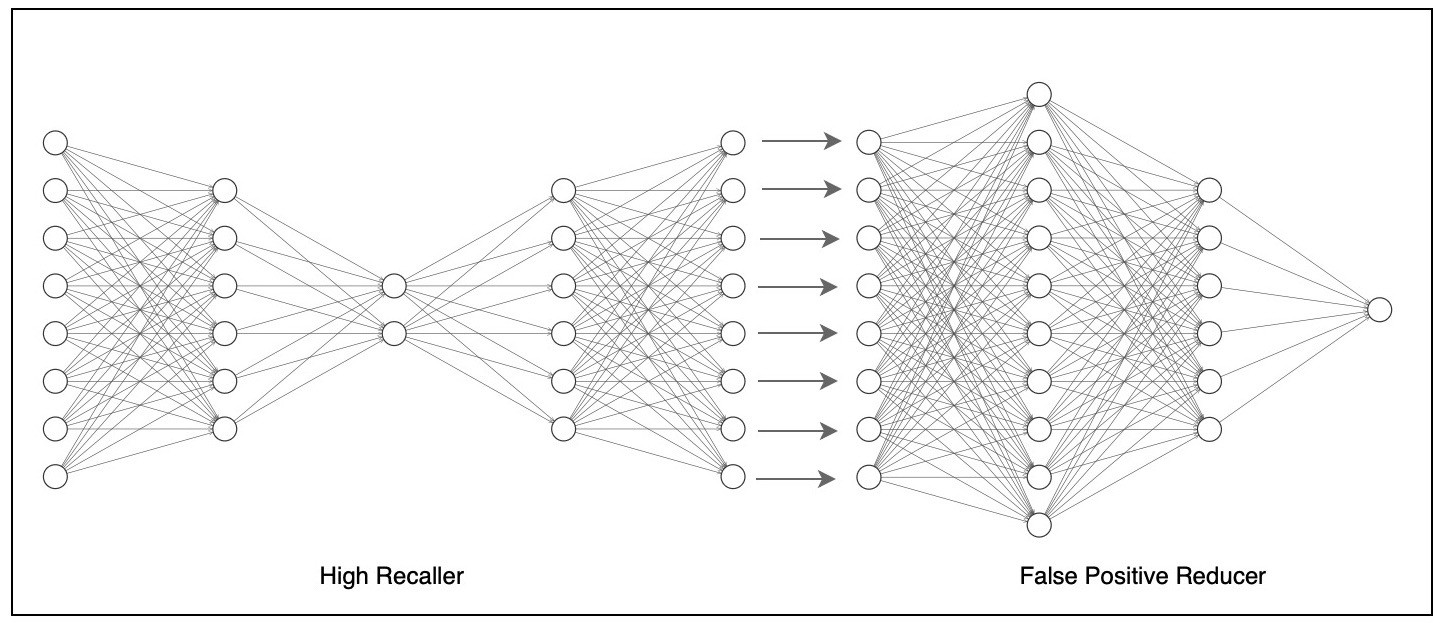
\includegraphics[width=\linewidth]{images/highrecaller.jpeg} 
         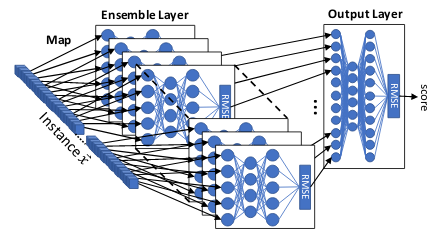
\includegraphics[width=\linewidth]{images/kitsune.png} 
      \end{column}
      \end{columns}

      
      
     \end{frame}
     
     \begin{frame}{Casos reales en mantenimiento predictivo}
      \begin{fullpageitemize}
         \small
         \item \textcolor{colordgray}{Chen, Z., \& Li, W. (2017). }Multisensor feature fusion for bearing fault diagnosis using sparse autoencoder and deep belief network. \textcolor{colordgray}{IEEE Transactions on Instrumentation and Measurement, 66(7), 1693-1702.}
         \item \textcolor{colordgray}{Jiang, G., He, H., Xie, P., \& Tang, Y. (2017). }Stacked multilevel-denoising autoencoders: A new representation learning approach for wind turbine gearbox fault diagnosis. \textcolor{colordgray}{IEEE Transactions on Instrumentation and Measurement, 66(9), 2391-2402.}
         \item \textcolor{colordgray}{Sun, W., Shao, S., Zhao, R., Yan, R., Zhang, X., \& Chen, X. (2016). }A sparse auto-encoder-based deep neural network approach for induction motor faults classification. \textcolor{colordgray}{Measurement, 89, 171-178.}
         \item \textcolor{colordgray}{Gugulothu, N., TV, V., Malhotra, P., Vig, L., Agarwal, P., \& Shroff, G. (2017). }Predicting remaining useful life using time series embeddings based on recurrent neural networks. \textcolor{colordgray}{arXiv preprint arXiv:1709.01073.}
         %\item Verma, N. K., Gupta, V. K., Sharma, M., \& Sevakula, R. K. (2013, June). Intelligent condition based monitoring of rotating machines using sparse auto-encoders. In 2013 IEEE Conference on Prognostics and Health Management (PHM) (pp. 1-7). IEEE.
      \end{fullpageitemize}
     \end{frame}
     
     \framecard[colororange]{{\color{white}\hugetext{EN RESUMEN\dots}}}
     
     \begin{frame}{En resumen\dots}
      \begin{fullpageitemize}
        \item Un autoencoder encuentra representaciones de forma no supervisada     
        \item Se adapta a multitud de casos de representation learning
        \item Detecta anomalías conociendo solo casos normales
      \end{fullpageitemize}
     \end{frame}
     
     % \framepic[0.8]{images/skeleton}{
     %  \begin{textblock}{7}(7,2.5)
     %     {\color{colorblue}\hugetext{\textbf{RUN!}}}
     %  \end{textblock}
     % }

    \input{templates/end-template}
\end{document}